\chapter{Background}   \label{ch:background}
\graphicspath{{Background/figures/}}

In the last few years, an increasing interest in event domain has led to diverse contributions in research. In this chapter, we provide a background analysis on the definition of ``\emph{event}'' in the Social Web and on the perceived qualities of available event directories. Then, we overview the Semantic Web technologies considered as powerful means to ensure a large scale data integration. Finally, we present some evaluation metrics used throughout this thesis.

\section{Events on the Web}   \label{sec:events-web}
An ever increasing amount of event-centric knowledge is spread over multiple social services, either materialized as calendar of events or illustrated by cross-media documents. Determining what an event is and how people use those services are two important research questions. In this section, we present the event definition adopted in this thesis, and we provide an overview of some social services as well as the perceived benefits and drawbacks of using them.

\subsection{Event Definition} \label{sec:events-def}
\emph{What is meant by the word ``event''?} has always been a research question leading to several meanings. This subject has received substantial consideration across different fields such as philosophy~\cite{Casati:2010} and computer science~\cite{Allan:1998}. From a broader point of view, a real event is considered as something that happens: a happening, an occurrence, an event~\cite{Scholes:1980}. This definition has been extended in a philosophical study to characterize events as an abstract concept in which the meaning depends on the target type such as activity, state or action~\cite{Casati:2010}. From technical point of view, an earlier work in Topic Detection and Tracking (TDT) field defines an event ``as something that happens at a particular time and place''~\cite{Allan:1998}. This definition puts emphasis on the spatial-temporal aspect, which seems to be adopted by many other researchers~\cite{Li:SIGIR05,Zhang:SIGIR07}. However, while events can happen at a specific time, other events continue over a long period of time. Moreover, associating a specific location to events fails to handle some events which may happen in different venues. These facts have led to other definitions in the literature attempting to cast an event to just a temporal entity~\cite{Rattenbury:SIGIR0} or to stress on the geographical dimension~\cite{Smith:SIGIR02}. To sum up, by drawing together all these definitions, three important views appear to identify what an event is. These views are represented by three \emph{Ws} questions: \emph{what}, \emph{when} and \emph{where}.

Later on, some researchers point out a missing concept that could define an event. They attempt to pay attention to ``\emph{who}'' was involved in the event. Although events can happen without participants, it seems important to consider this aspect when it comes to describe the people's experiences. Thus, the definition in~\cite{Allan:1998} has been extended to ``an event is something that has a specific time, location, and people associated with it''~\cite{Allan:2002}. For instance, it has been shown that the ``\emph{who}'' view is important to define a historical event which is described by five elements: object, person, location, time and cause~\cite{Nakahira:WWW07}. While causality appear in some definitions, it is of less significance to our work since we are not primarily interested in linking events by cause/effect relationships. 

In~\cite{Shaw:ASWC09}, the authors proposed a study to compare existing models that attempt to represent events in a structured format. They propose an interoperable model to represent
intersubjective ``consensus reality'' over all event definitions. Based on this model, we define an event in terms of the four \emph{Ws} questions as follows:

\begin{enumerate}
\item \emph{What} happened: represented by a set of terms.
\item \emph{Where} it happened: associates an event with any number of places.
\item \emph{When} it happened:  associates an event with a specific time or period of time.
\item \emph{Who} was involved: distinguishes between people having ``active'' or ``passive'' role.
\end{enumerate}

\subsection{Social Websites}
Events on the Web exist in two different types: \textit{unstructured} and \textit{structured}. Unstructured events are mostly represented in form of natural language phrases which require complex parsing and extraction mechanisms. On the other hand, structured events are represented in a well-defined structure that may differ from one site to another. Currently, there exists a large variety of websites that host structured information about past and upcoming events, some of which may display media. In this thesis, we focus on structured events as provided by some popular event websites. In the following, we provide an overview about these sites as well the platforms which host related media.

\myparagraph{Event Sites}  
Many Web services available online aim to help users search and share information about past and upcoming events. Whilst some websites focus on a specific type of events (e.g. musical, conference), other ones provide a wide span of different types including film, theater, exhibition, etc. In this thesis, we use some popular event sites described as following.  

\begin{itemize}
 \item \textbf{Last.fm\footnote{\url{http://www.last.fm}}:} is the largest music based platform founded in 2002 having more than 30 million active users. It allows to build a user profile based on listening preferences of music collection or radio station. In October 2006, Last.fm incorporated a system that lets users post musical concerts with some details (date, venue, location, artists, etc.).  They are also able to express their intent to attend events using RSVP (e.g. \emph{I'm going}). Tags and 
comments are also possible on almost any item such as a user, event, artist, or track. Finally, users can register in any group which may be linked to artists or countries, and can add other users as friends. Figure~\ref{fig:lastfm} depicts the homepage of Last.fm.

\begin{figure}[htbp]
  \centering
  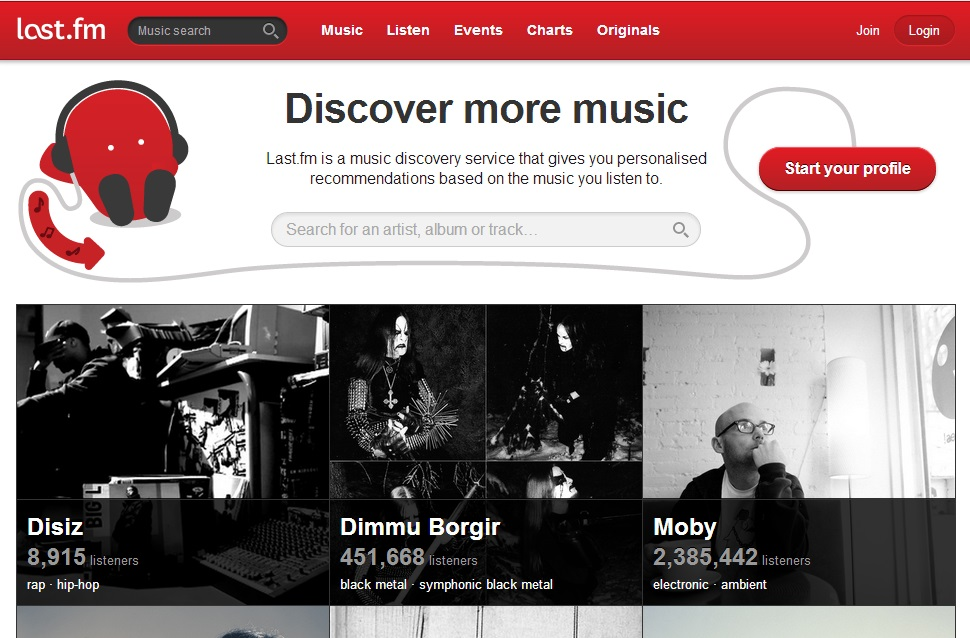
\includegraphics[scale=0.41]{lastfm.jpg}
  \caption{Last.fm}
  \label{fig:lastfm}
\end{figure} 
  
 \item \textbf{Eventful\footnote{\url{http://www.eventful.com}}:} is a popular event-based service founded in 2004. It boasts one of the world's largest databases of events having a wide variety of types such as sport, cinema, family, education and other local entertainment. It allows users searching for events by location, time, category, artist and descriptive keyword. It also provides functionality to view and manage a list of favorite artists and venues. Figure~\ref{fig:eventful} depicts the homepage of Eventful.
 
  \item \textbf{Lanyrd\footnote{\url{http://www.lanyrd.com}}:} was founded in 2010 providing a social directory of conferences and other professional events. It enables users to enter location, speakers, schedule and other descriptive details. Users can be identified through the Twitter\footnote{\url{http://www.twitter.com}} or LinkedIn\footnote{\url{http://www.linkedin.com}} API and are invited to list the conferences which they are attending or speaking at. Figure~\ref{fig:lanyrd} depicts the homepage of Lanyrd.
 
 \begin{figure}[H]
   \centering
  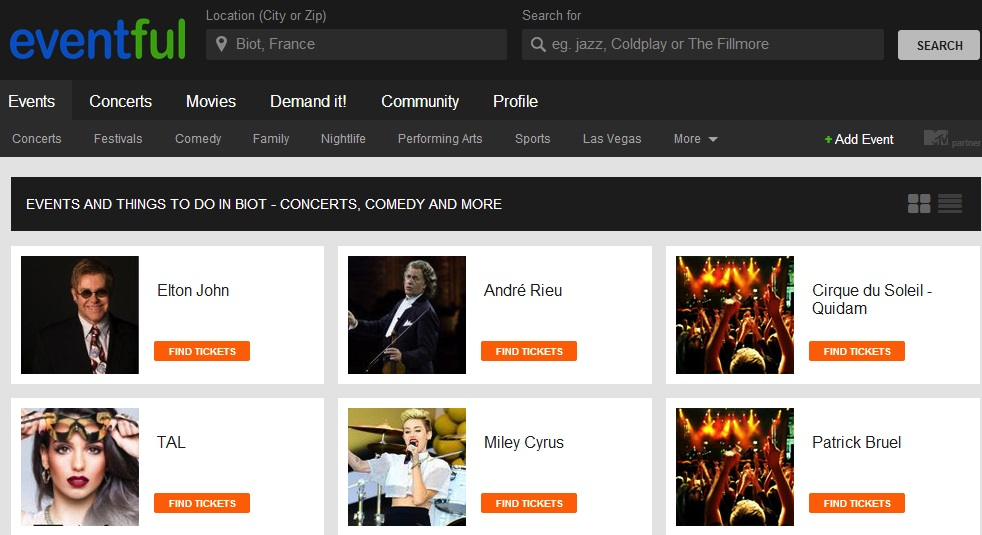
\includegraphics[scale=0.3]{eventful.jpg}
  \caption{Eventful}
  \label{fig:eventful}
 \end{figure} 
 
  \begin{figure}[H]
   \centering
  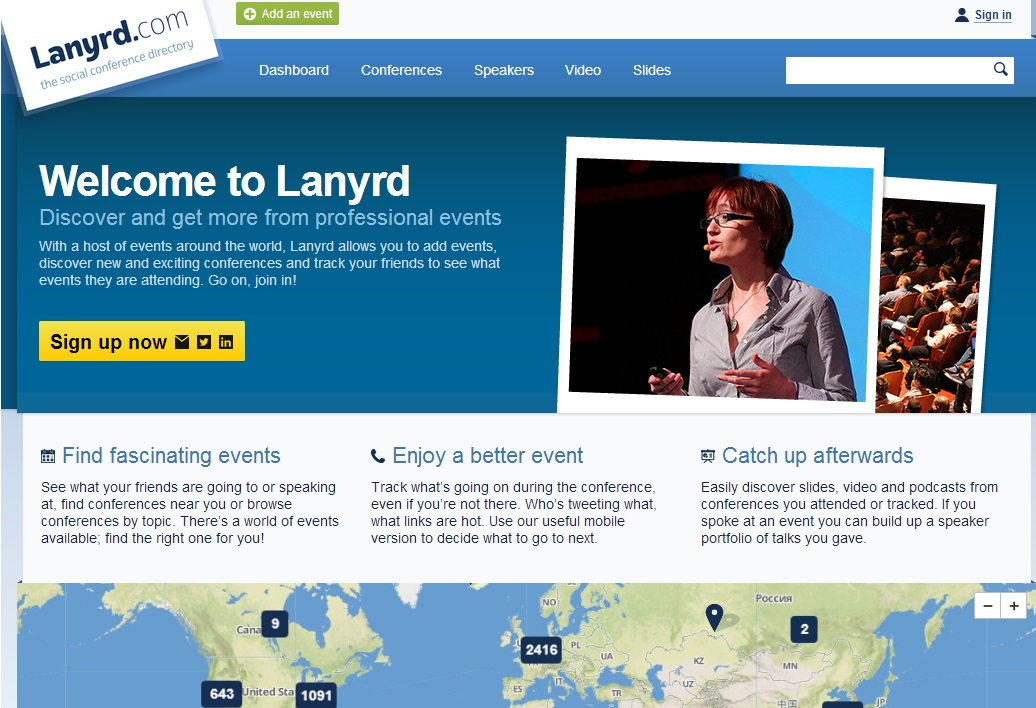
\includegraphics[scale=0.3]{lanyrd.jpg}
  \caption{Lanyrd}
  \label{fig:lanyrd}
  \end{figure} 
  
 \begin{figure}[H]
   \centering
  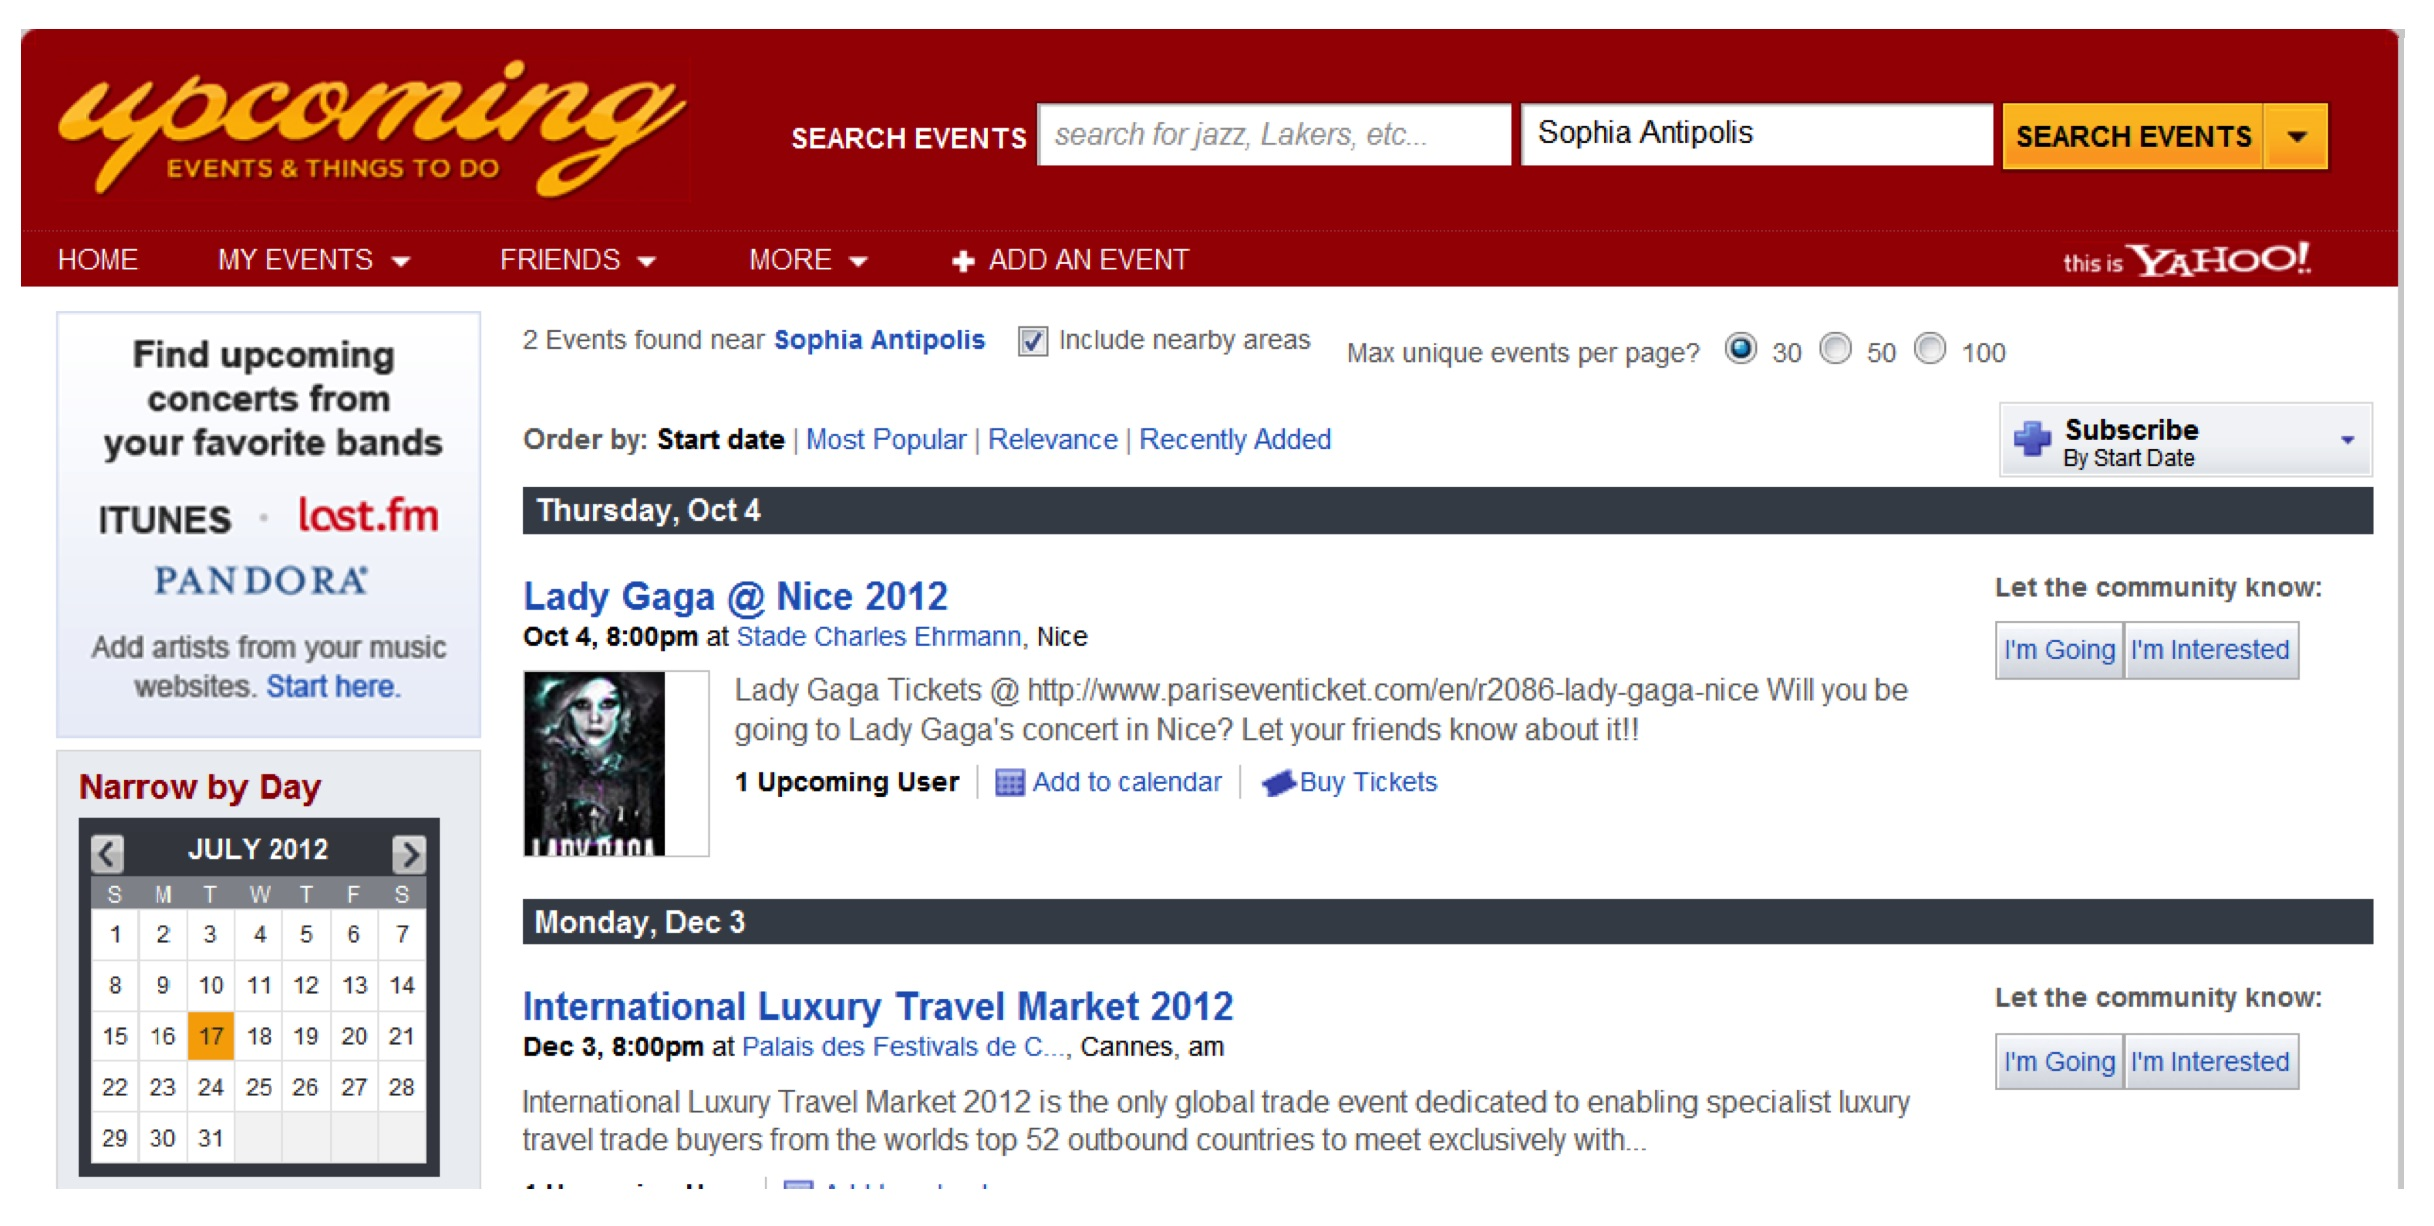
\includegraphics[scale=0.13]{upcoming.jpg}
  \caption{Upcoming}
  \label{fig:upcoming}
  \end{figure}   
 
   \item \textbf{Upcoming:} was another event-based service launched in 2003, acquired
by Yahoo! in 2005 but retired in 2013. It was a competitor of Eventful and offers similar functions. Upcoming hosted different types of events such as conferences, art exhibitions along with useful details including time, location, etc. Users can create and manage events and have a ``friend'' relationship with each other. Figure~\ref{fig:upcoming} depicts the homepage of Upcoming.

\end{itemize}

\myparagraph{Media Sites} Many participants use social media platforms to engage in discussions with comments, and share media captured during events. In the following, we describe some popular media sites involved in this thesis.  


\begin{itemize}
\item \textbf{Flickr\footnote{\url{http://www.flickr.com}}:} is one important photo and video sharing website founded in 2004. The site claimed 6 billion of hosted photos in 2012 witnessing a significant growth in the past few years. It provides rich data about photos that have been widely exploited by research community. This data describes several attributes such as title, description, uploading time, geo-coordinates, tags, etc. One popular attribute is the so-called ``machine tag'' or ``triple tag'' which is used in this thesis. It is based on a special syntax which is meaningful to be processed by machines. It comprises three parts: (1) the namespace to denote the classification of a tag ('flickr', 'geo', etc.); (2) the predicate to represent the property of the namespace; (3) and the value of the tag. For instance, "geo:lat=25.070173" is a tag for the geographical latitude whose value is 25.070173.

\item \textbf{Twitter:} is the most famous micro-blogging service emerged in 2006. The site claimed 200 million of active users in February 2013. It allows users and organizations to publish text messages limited to 140 characters. These status messages are called ``tweets'' or more generally ``microposts'' and the subscribers are called ``followers''. Users can also reply or ``retweet'' messages. Retweets can be comparable to forwarded emails indicated by ``RT'' character. Moreover, a message can contain a sort of tag preceded by the hash character which is known as a ``hashtag'' e.g. \#tag. Finally, users have the option to follow other users, thus becomes a ``followee'' of them.

\end{itemize}

\subsection{Exploratory User Study}
The initial motivation behind this thesis lies in an exploratory user-centered study conducted by Fialho et al.~\cite{Fialho:EVENTS10}. The goal is to understand the event-related activities (e.g. searching, attending, sharing) and to collect insights about existing Web-based technologies. This study consisted of a user survey completed by 28 participants and two focus-group sessions (10 and 25 participants). The questions were elaborated to assess the perceived benefits and drawbacks of using: event directories, media directories, social networks, and a merger of these services.

\myparagraph{Finding and attending an event} Participants reported to discover events mainly through invitations, recommendations, friends' posts or some traditional media (e.g. news articles, ads, etc). They also refer to previously attended events or venues to find new events, and they use search engines particularly when they knew what to look for. Moreover, it is found that decision about attending an event seems to prioritize some significant constraints such as time, location and price. Social information about which friends will attend an event has also an important role in decision making. Other additional details appear to have slight influence like the case of subjective factors (type, topic, performer). To share their experiences, participants tend to use media directories and social networks by posting comments, photos and few videos. 

\myparagraph{Use of social directories} According to participants, event directory is the best source to provide a general overview of an event context within a single channel. It also enables a user-friendly event exploration from various views (what, when, where) along with other features (e.g. tickets, comments). However, it appears that the information perceived are often incomplete and insufficient for decision support (lack of media and geographic map). To overcome this issue, media directories have been considered as one valuable outlet that better conveys the event environment based on visual information. Social network sites was also said to enhance event directories by adding communication and sharing features (e.g. comments, invitations) along with other useful details (e.g. attendance, popularity). Besides, some other functionalities have been mentioned to be desirable for reducing the information overload. One functionality supports the event recommendation based on friend's attendance and user interests. Another functionality is to better visualize events by improving search features (e.g. geographic map) and enriching descriptions (e.g. price, attendance).

\myparagraph{Recapitulation} TO sum up, lack of coverage of event directories and frustration of being locked in a particular site are the recurrent issues perceived during the study. Participants recognized that there is a need to access several social channels to gather information. One participant reported ``\textit{I don't like always having to go from one site to another to find out things about the event}''. Overall, users advocate the need for a single source to explore events, not by creating another information source, but by centralizing all available information leading to broader coverage. In addition, they highlight the role of photos and videos to provide powerful means of identifying several event characteristics. Media is thus useful to convey the experience and to support decision making. Nevertheless, a common concern of information overload suggests that the environment should avoid cluttered information and provide browsing and recommendation options. Motivated by this study, we decided to build a platform based on Semantic Web technologies in order to integrate information spread in many silos and thus enhance the event coverage.

\section{Events in Research}       \label{sec:events-research}
In the last few decades, a growing corpus of research has been centered on the notion of ``\emph{event}''.  Such particular attention sheds light on the inherent complex nature of events. This is behind the fact that even the definition of what an event is fails to reach a real consensus. Recently, the growth of social networks along with the technological improvements that made connected devices easy to use, made the user-contributed Web a primary source of information about any kind of real world happening. Studying events on the Web has been the subject of an attractive diversity of research works. Summarizing the various challenges surveyed in these studies, we discern three major key aspects that will drive our strategy to design relevant program or system.

An event is an entity that handles in essence contextual dimensions, each of which is related to one attribute such as time, location, topic and participants. This multi-faceted aspect has driven the design of many programs which aim, for example, to detect events from social media~\cite{Allan:1998,Weng:ICWSM11} or to explore meaningful relationships between them~\cite{Corda:IESD12}. Recently, a research study proposed by Ramesh Jain~\cite{Jain:2007} explored the multi-dimensionality to introduce a coherent definition of the so-called ``\emph{Web of events}''. Indeed, this term has been conceived as the Web in which nodes represent events having informational and experiential attributes with links describing its structure and relationships. Informational attributes provide descriptive metadata of events including title, location, participants, and so on. Experiential attributes describe the sensory data highlighting the event experience such as image and video. Various links can exist in the Web of events such as the one which connects events with experiential attributes. Other links may capture the natural relationships that exist among events such as identical, temporal and causal. Among all the dimensions, it appears that the temporal one has received a substantial attention in research. Several studies in TDT field have been based on time series analysis of media content to identify events. A typical example is the work of Weng et al.~\cite{Weng:ICWSM11} that considers an event as a burst of words in a specific time window. Another earlier work proposed by Allen et al.~\cite{Allen:1994} in AI field provides a logic model to represent the temporal relationships between pairs of events.

Also related to the temporal dimension, the second key aspect is the short event lifetime. Broadly speaking, an event is an ephemeral item that only exists between two time instants. This period seems also to be correlated with peaks of users' activities in social networks where people engage in discussions about this event. Such transiency has constrained the design of many real-time systems which should support high scalability and online processing of streaming data. For example, Sakaki et al.~\cite{Sakaki:WWW10} proposed a real-time system to identify earthquake events in Twitter. Becker et al.~\cite{Becker:ICWSM11} used an online clustering technique to detect in real-time groups of topically similar tweets that correspond to events. Another system perceived to suffer from the fleeting nature of target items are those which provide personalized recommendations. Unlike classic item (movie, book) recommendation, the system can only acquire a limited history about event participation which induces highly sparse rating data. This is a well-known problem in a recommender system appearing when an item has not received enough ratings to be meaningfully used. Such items require an advanced recommender system such as the one proposed by Cornelis et al.~\cite{Cornelis:IICAI05} based on the hybridization of existing and popular recommendation techniques (e.g. collaborative filtering, content-based).

The third key aspect is the social information that an event holds. In reality, people regularly attend various events or share their experiences, thus forming a dynamic space of rich social interactions. As such, social networks can be directly constructed from event-centric user activities which can be offline in the physical world or online on the Web. These so called \textit{event-based social networks} have been studies in some research works. For example, Liu et al.~\cite{Liu:2011} proposed a formal definition of an event-based social network, and they extensively studied its underlying properties along with community detection and information diffusion. Liao et al.~\cite{Liao:CIKM13} used them to reveal the latent social relations among users and the implicit users' preferences which are exploited in event recommendation.

\section{Semantic Web}       \label{sec:sematic-web}
The current Web, as introduced by Tim Berners-Lee in 1989, is a huge information space mostly represented in interlinked HTML documents. While the interpretation of this information is delegated to human beings, computers serve merely as storage and communication platform. This fact prevents machines from achieving many tasks based on automated data processing such as search and query answering. 

As has has been designed for human consumption, the Web still needs a high human involvement to interpret, combine and categorize data. To overcome this limitation, many efforts have been spent in some fields such as Information Retrieval, Machine Learning, and Natural Language Processing (NLP). They have produced complex systems trying to automatically extract meaning from unstructured data. Typical examples are the search engines such as Yahoo\footnote{\url{http://www.yahoo.com}} and Google\footnote{\url{http://www.google.com}}. They mainly rely on NLP routines to index data without any knowledge about the meaning of the terms and the relationship between them. Although the emergence of these search engines was a success for the Web, there is still a semantic gap between what the machine understands and what the user knows about the data~\cite{Mika:07}. This is where Semantic Web intervenes trying to fill the knowledge gap. In this context, Berners-Lee et al.~\cite{BernersLee:01} provide the following definition:

\begin{quote}
\emph{The Semantic Web is not a separate Web but an extension of the current one, in which information is given well-defined meaning, better enabling computers and people to work in cooperation.}
\end{quote}

How to expand a Web of documents for users with a Web of information for machines is the vision of the Semantic Web. The objective is to automate the human data processing without using full-fledged NLP or reasoning methods by giving meaning to resources and linking them. In the Semantic Web, an intelligent document has awareness about its own content, making it exploitable by automatic process. This way will enable machines to answer complex queries which are currently not possible without human involvement. For example, one user may want to find an event that will take place next weekend in Nice covering one specific topic and with suitable price. For this, he/she currently needs to trawl through various websites and look at different fields (e.g. location, topic, price). On the contrary, the answer in the Semantic Web can be provided by an intelligent Web agent that decodes the query and exploits linked data to deliver relevant information.

To realize this vision, a series of technologies and standards have been proposed. They provide ability to add meaning to the Web content and to represent it in a machine understandable format. In the following, we describe some of these standards along wit the trend of Linked Data.

\subsection{Resource Description Framework (RDF)}
Resource Description Framework (RDF)~\cite{Lassila:1999} is a recommendation of the World Wide Web Consortium (W3C) that describes the Web resources. In the Semantic Web, a resource is anything that has an identity and it can be a person, document, image, location, etc. Each resource is assigned a Universal Resource Identifier (URI)~\cite{Berners:2005} which is a formatted string to identify an abstract or physical resource. A common type of URI is the Universal Resource Locator (URL) used to identify resources located on the Web.

RDF is originally designed as a simple metamodel for describing information in a direct graph with labeled nodes and arcs. In this model, the nodes represent the Web resources and the arcs represent the properties which link together these resources. Note that a property is a specific aspect, characteristic, attribute, or relation used to 
describe a resource~\cite{Lassila:1999}. In RDF, resources can be described and linked by a set of statements forming a graph, also known as a semantic network. Each statement is a triple which is usually denoted as $<s,p,o>$ and composed of:
\begin{itemize}
\item Subject: the resource which the statement refers to. It is identified by a URI.
\item Predicate: describes a property of the subject and expresses the relationship between the subject and the object.
\item Object: specifies the value of the property. It can be a resource identified by a URI or an atomic value named literal. Note that a literal can be plain or typed. A plain literal
is a string combined with an optional language tag (e.g. "thesis"@en). A typed literal is a string associated with a datatype URI (e.g. "0.52"\char`\^\char`\^datatypeURI). The datatype URI
specifies the datatype of the literal which can be integer, float or date, as defined by the XML Schema Datatype specification\footnote{\url{http://www.w3.org/TR/xmlschema-2}}.
\end{itemize}

Figure~\ref{fig:rdffrance} depicts an example of RDF graph-based representation about ``France'' which is identified by a URI on the Web. Note that this URI identifies a subject resource which is assigned the type Country and has \emph{France} as label. 

 \begin{figure}[htbp]
   \centering
  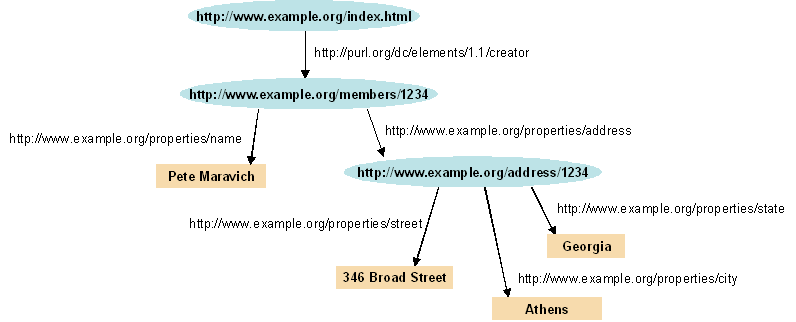
\includegraphics[width=\linewidth]{rdf.png}
  \caption{Example of RDF representation about France}
  \label{fig:rdffrance}
  \end{figure} 

Several methods exist for serializing the RDF data model. The most common format is RDF/XML. There exist other text-based formats introduced by W3C such as Turtle\footnote{\url{http://www.w3.org/TeamSubmission/turtle}} and N-Triples\footnote{\url{http://www.w3.org/TR/n-triples}} which are easier to read than RDF/XML. To query the RDF graph, W3C has defined a query language called SPARQL\footnote{\url{http://www.w3.org/TR/rdf-sparql-query}}. It contains triple patterns along with their conjunctions (e.g. logical ``and'') and disjunctions (e.g. logical ``or''). It also supports extensible value testing and constraining queries by named RDF graph.

\subsection{RDF Schema}

RDF is a very simple and flexible data model that allows users to describe resources using properties and values. However, it does not provide means to define vocabularies and to specify domain specific classes and properties. Hence, other terms are needed to describe the classes of resources and the relationship between them. As a solution, an extension of RDF called RDF Schema~\cite{Brickley:2014} provides a basic vocabulary to interpret RDF statements. RDFS vocabulary simply describes taxonomies of classes and properties and defines very basic restrictions.

In RDF Schema, URIs have as a namespace \url{http://www.w3.org/2000/01/rdf-schema#}      
conventionally associated with the prefix \emph{rdfs:}. In summary, (1) A resource is an instance of one class (\emph{rdfs:class}) or more classes where classes are organized in a hierarchy using \emph{rdfs:subClassOf} property; (2) Properties have as class \emph{rdf:Property} and are organized in a hierarchy using \emph{rdfs:subPropertyOf}. Some restrictions on properties are specified such as \emph{rdfs:domain} to define the class of the subject, and \emph{rdfs:range} to define the class of the object. 

\subsection{Ontology Vocabulary}
RDF and RDF Schema both have limited expressivity. While RDF describes a simple way to represent structured data, RDF Schema only provides basic hierarchies associated with simple restrictions. However, there is a need for more expressivity to be able to define a formal explicit description of concepts in some complex domains. Therefore, the concept of ontology has been adopted as an extension of RDF Schema with more expressive constructs. Ontology was originally defined by Artificial Intelligence (AI) community as explicit formal specification of a conceptualization in domain of interest~\cite{Gruber:1993}. It typically describes the concepts of the domain and the semantic interconnections that hold between them, along with some logic and inference rules. In general, ontology is the reflection of a shared and common  understanding of a domain that can be communicated between people and/or machines. For example, given the different websites containing event information, the use of common ontology will enable Web agents to aggregate data and to answer more complex user queries. In the following, we list some core elements of an ontology:

\begin{itemize}
\item Class: defines a concept, type or collection in a specific domain. It groups objects that share some properties and are organized in a hierarchy. For instance, in a university domain, the class Student is more specialized than the class Person.
\item Individual: also known as instance or object and is a member of a class. For instance, \emph{Nelson Mandela} is an instance of the class Person.
\item Property: is a binary relation to describe how classes and individuals can be related to each another. There is datatype property which connects instances with RDF literals, and object property which connects instances of two classes. For example, \emph{hasFather} is an object property that can relate two instances of the class Person.
\end{itemize}

To model ontologies, the Web Ontology Language (OWL)~\cite{OWL:2012} is the current markup language endorsed by W3C. Compared with RDF and RDFS, OWL defines a vocabulary with additional formal semantics. It provides more relations between classes (e.g. \emph{disjointWith}), logical properties (e.g. \emph{intersectionOf}, \emph{sameAs}) and enumerations (e.g. \emph{oneOf}, \emph{allValuesFrom}), among others.

\subsection{Linked Open Data}

The Semantic Web is predicated on the availability of large amount of structured RDF data, not in isolated islands but as a Web of interlinked data. A major milestone to realize this vision is the Linked Open Data (LOD or Linked Data) project~\cite{LOD:2011} that connects RDF datasets on a large scale. LOD captures a growing knowledge from various domains forming an open ``Web of Data'' freely available to access, download, and use. Today's LOD comprises billions of RDF triples counting millions of links between data sources. Formally, Linked Data has been defined as about ``data published on the Web in such a way that it is machine readable, its meaning is explicitly defined, it is linked to other external datasets, and can in turn be linked to from external datasets''~\cite{Bizer:HB09}. 
  
Linked Data follows the principles outlined by Tim Berners-Lee to publish information on the Web, which are:

\begin{itemize}
\item Use URIs as names for things
\item Use HTTP URIs so that people can look up those names.
\item When someone looks up a URI, provide useful information, using the standards (RDF, SPARQL)
\item Include links to other URIs. so that they can discover more things.
\end{itemize}

Overall, these principles stress on the accessibility and the linkage of data that adhere to the architecture and standards of the Web. Figure~\ref{fig:lod} shows the significant number of published datasets in 2011, covering information from diverse areas such as encyclopedic, government, geographic, entertainment, publications and so on.  For instance, DBpedia\footnote{http://dbpedia.org} is one of the largest RDF repository in the Linked Data focusing on extracting multilingual knowledge from Wikipedia. At the time of writing, the English edition of DBpedia consists of 470 millions RDF triples that describe 4.0 million things covering a wide range of topics, and contains 45 million RDF links to several hundred external datasets.

 \begin{figure}[htbp]
   \centering
  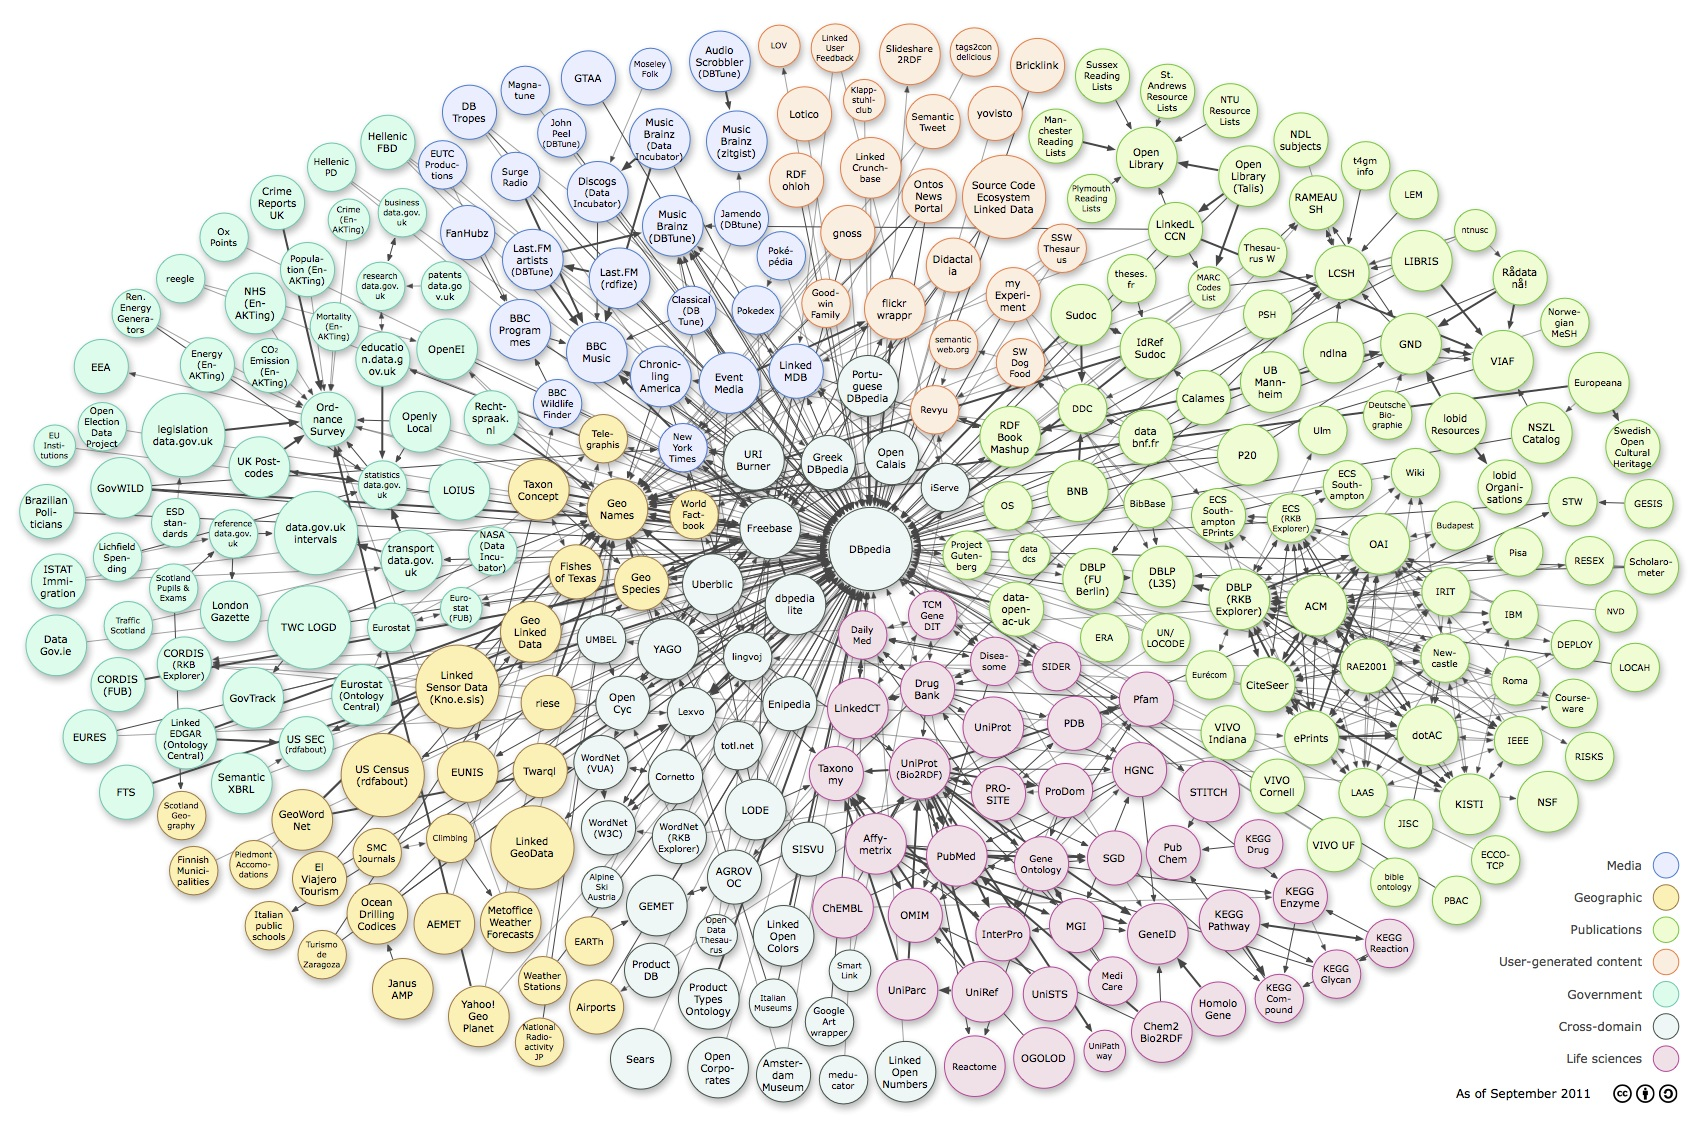
\includegraphics[width=\linewidth]{lod.jpg}
  \caption{Linked Open Data (LOD) Cloud in September 2011}
  \label{fig:lod}
 \end{figure} 

Client applications can access and use RDF links to navigate between datasets and to discover additional information. In order to be part of Linked Data, datasets need to create links to related instances in other datasets. To cope with the large amount of instances, it is a common practice to draw on automated or semi-automated tools or methods to generate links between data sources. Yet, this is still a challenging task and significant research efforts have been devoted to address it.

\section{Evaluation Metrics} \label{sec:evaluation-metric-back}
In this section, we overview the mostly used evaluation functions in this thesis namely, Precision, Recall and F-score. These measures are widely exploited in data reconciliation field. For a reconciliation task, results can be classified into 4 categories which are: \textit{true positives (tp)}, \textit{true negatives (tn)}, \textit{false positives (fp)} and \textit{false negatives (fn)}. The terms \textit{positive} and \textit{negative} refer to the system's prediction, and the terms \textit{true} and \textit{false} refer to whether this prediction is correctly corresponding to the ground truth. Precision computes the percentage of correctly matched reference pairs (tp) over all matched reference pairs (tp and fp) (Equation~\ref{eq:precision}). Recall computes the percentage of correctly matched reference pairs (tp) over pairs of references in the ground truth (tp and fn) (Equation~\ref{eq:recall}).

\begin{equation} \label{eq:precision}
Precision= \frac{tp}{tp+fp}
\end{equation}

\begin{equation} \label{eq:recall}
Recall= \frac{tp}{tp+fn}
\end{equation}
\\
\\
In practice, F-score is also popularly used and it combines both precision and recall:

\begin{equation*}
F\textrm{-}score= 2 \cdot \frac{precision \cdot recall}{precision+recall}
\end{equation*}

\section{Conclusion}   \label{sec:conclusion}
In this chapter, we first reviewed several definitions given to the concept of event and we adopted an interoperable definition that describes essential aspects. Then, some popular social websites hosting event related data have been described. The drawbacks perceived by people to use these websites particularly motivated us to carry out this work. Finally, we detailed the fundamentals of the Semantic Web and the evaluation criterion which will be involved in this thesis.







